\documentclass{jreport}
\usepackage[dvipdfmx]{graphicx}
\usepackage{float}
\usepackage{xcolor}
\usepackage{amsmath}
\usepackage{amsfonts}
\usepackage{amssymb}
\usepackage{amsthm}
\usepackage{bm}
\usepackage{romannum}
\usepackage[dvipdfmx,hidelinks]{hyperref}
\usepackage{pxjahyper}
\usepackage{framed}
\usepackage{pifont}
\newenvironment{claim}[1]{\par\noindent\underline{Claim:}\space#1}{}
\newenvironment{claimproof}[1]{\par\noindent\underline{Proof:}\space#1}{\hfill $\square$}
\DeclareMathOperator{\spn}{\mathbb{Q}-span}
\begin{document}
\pagenumbering{arabic}
\title{第三回レポート問題}
\author{習近平}
\maketitle
\setcounter{chapter}{3}
\newpage
\tableofcontents
\addcontentsline{toc}{chapter}{目次}
\newpage
\section{ばねで結合した振り子の連成振動を議論しよう}
\subsection{1}
\begin{equation}
	\left\{
	\begin{aligned}
		M\frac{d^2x_n}{dt^2} &= -k(x_n -x_{n-1}) + k(x_{n+1} -x_n) -T\sin \theta_n \\
		M\frac{d^2y_n}{dt^2} &= T\cos \theta_n -Mg =0
	\end{aligned}
	\right.
\end{equation}
\begin{equation}
	M\frac{d^2x_n}{dt^2} = -k(2x_n-x_{n-1}-x_{n+1})-\frac{Mgx_n}{l}
\end{equation}
\subsection{2}
代入して、整理すると次のように定まる:\\
\begin{equation}
	A_n = \frac{k}{2k-M(\omega^2 - g/l)} (A_{n-1} +A_{n+1})
\end{equation}
\subsection{3}
仮定の解を先程の等式の右辺に代入し、三角函数の和積の公式を適用すると次の式が得られる:\\
\begin{equation}
	\begin{aligned}
	  A_n &= \frac{k}{2k-M(\omega^2 - g/l)} (A_{n-1} +A_{n+1})\\
	      &= \frac{k}{2k-M(\omega^2 - g/l)} (\sin (p(n-1)) +\sin (p(n+1)))\\
	      &= \frac{2k}{2k-M(\omega^2 - g/l)} A_n\cos p \\
	  \omega &= \sqrt{\frac{4k\sin^2(\frac{p}{2})}{M} + g/l}
	\end{aligned}
\end{equation}
\subsection{4}
仮定の解に$x_0=0$の初期条件から情報を得られず、$x_{N+1} =0$より、\\
\begin{equation}
	\begin{aligned}
	A_{N+1} &=\sin (p(N+1)) =0 \Rightarrow p =\frac{m \pi}{N+1} (m \in \mathbb{N}) \\
		\omega_m &=\sqrt{\frac{4k\sin^2 (\frac{m \pi}{2(N+1)})}{M} + g/l }
	\end{aligned}
\end{equation}
\subsection{5}
\begin{figure}[H]
	\centering
	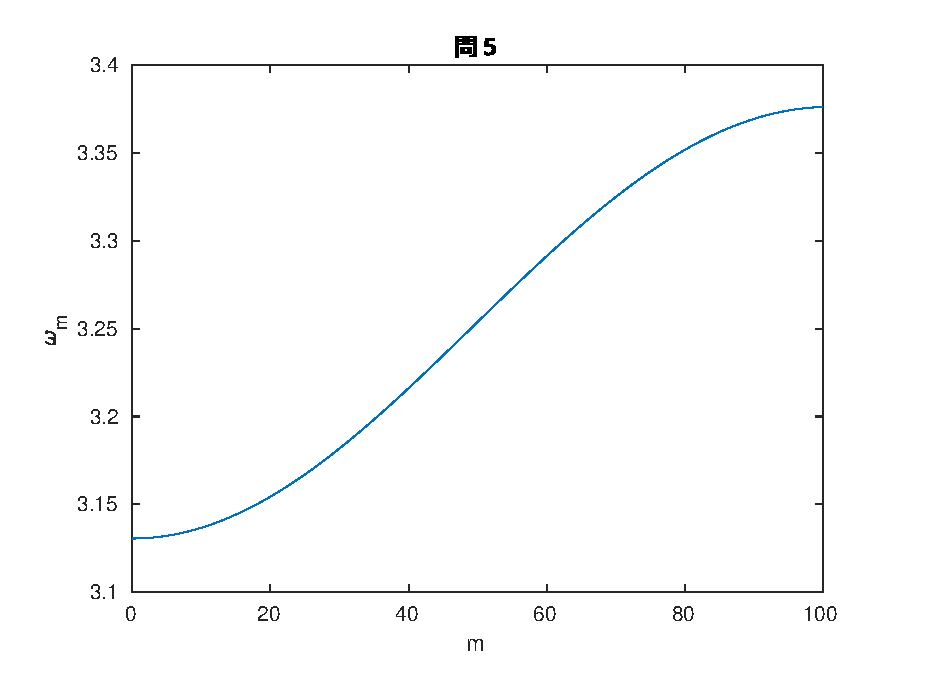
\includegraphics[width=8cm]{5.eps}
\end{figure}
\subsection{6}
\begin{equation}
	x_n(t) = \sum_{i=1}^{m} \sin (\frac{in\pi}{N+1}) \sin ( \omega_i t- \delta) 
\end{equation}
\subsection{7}
\begin{equation}
	\begin{aligned}
		M\frac{d^2x_n}{dt^2} &= -k (2x_n - x_{n-1} -x_{n+1} ) -\frac{Mgx_n}{l}\\
		\frac{\partial^2 u(x,t)}{\partial t^2} & =\frac{kc^2}{M} \cdot \frac{\partial^2 u(x,t)}{\partial x^2} -\frac{g}{l} \cdot u(x,t) \\
		\frac{\partial^2 u(x,t)}{dt^2} &= -\omega_0^2 u(x,t) + v^2 \frac{\partial^2 u(x,t)}{\partial x^2}
	\end{aligned}
\end{equation}
\subsection{8}
\begin{equation}
	\begin{aligned}
		-\omega^2 u(x,t) &= -\omega_0^2 u(x,t) - k^2 v^2 u(x,t)\\
		-\omega^2 &= -\omega_0^2 -k^2 v^2\\
		w&= \sqrt{\omega_0^2 + k^2v^2}
	\end{aligned}
\end{equation}
\subsection{9}
\begin{equation}
	\left\{
	\begin{aligned}
		kx + \alpha &=0 \\
		kc(N+1) &= m \pi 
	\end{aligned}
	\right.
\end{equation}
\begin{equation}
	\begin{aligned}
		kc &=\frac{m \pi}{N+1} \\
		\omega &= \sqrt{\omega_0^2 +\frac{k(\frac{m \pi}{N+1})^2}{M}}
	\end{aligned}
\end{equation}
\subsection{10}
\begin{figure}[H]
	\centering
	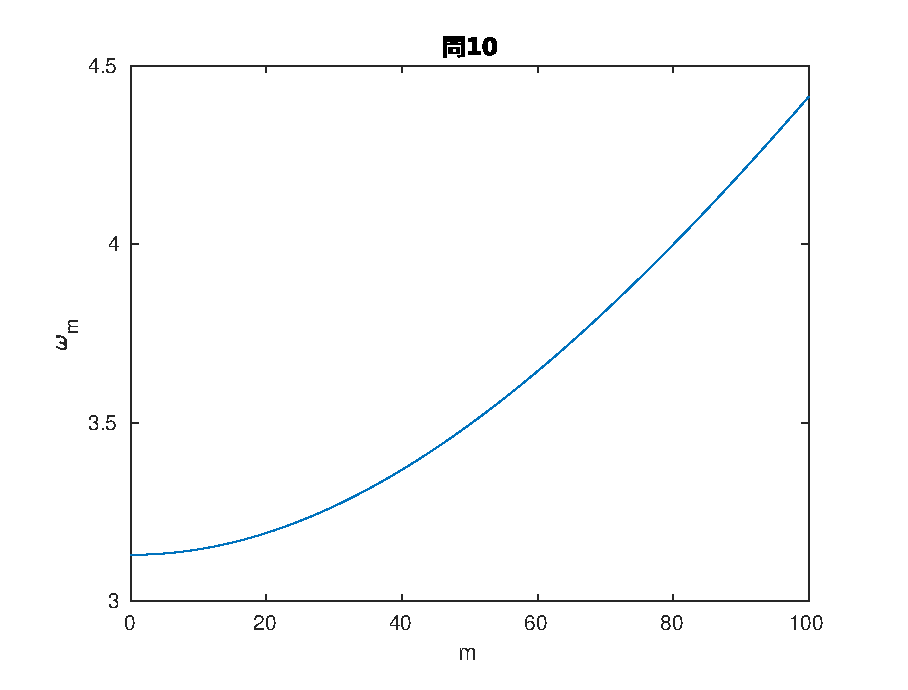
\includegraphics[width=8cm]{10.eps}
\end{figure}
\subsection{11}
\begin{equation}
	\sum_{i=0}^m A \sin (kx) \cdot \sin \left( \sqrt{\omega_0^2 +\frac{k(\frac{i\pi}{N+1})^2}{M}} t -\delta \right)
\end{equation}
\newpage
\section{問題2}
\subsection{1}
\begin{equation}
	\begin{aligned}
		\sum_{m=1}^{\infty} \sin (m \pi \frac{x}{l} ) \frac{d^2 Q_m (t) }{dt^2} &= - \sum _{m=1}^{\infty} (\frac{m \pi v}{l})^2 \sin(m \pi \frac{x}{l})Q_m(t) \\
		\sum_{m=1}^{\infty} \int_0^l \sin(n \pi \frac{x}{l} ) \sin (m \pi \frac{x}{l} )dx \cdot \frac{d^2 Q_m (t) }{dt^2} &= - \sum _{m=1}^{\infty}\int_0^l (\frac{m \pi v}{l})^2 \sin(n \pi \frac{x}{l} )\sin(m \pi \frac{x}{l})dx\cdot Q_m(t) \\
		\frac{d^2 Q_n(t)}{dt^2} &=-\omega_n^2 Q_n(t)
	\end{aligned}
\end{equation}
	ここで、$n$を$m$とおけばよい。
\subsection{2}
\begin{equation}
	\begin{aligned}
		Q_m(t) &= A_m \sin(\omega_m t - \delta_m)\\
		u(x,t) &= \sum_{m=1}^{\infty} A_m \sin (m \pi \frac{x}{l} ) \sin(\omega_m t - \delta_m)
	\end{aligned}
\end{equation}
\subsection{3}
\begin{equation}
	\begin{aligned}
		K&=\sum_n \frac{M}{2}\left(\frac{du_n}{dt}\right)^2\\
		 &=\frac{\rho}{2} \int_0^l \left( \frac{\partial u(x,t)}{\partial t} \right) ^2dx
	\end{aligned}
\end{equation}
\subsection{4}
\begin{equation}
	\begin{aligned}
		U &= \sum_n Tc \left( 1 + \frac{1}{2} \left( \frac{u_{n+1} - u_n }{c} \right) ^2 -1 \right) \\
		  &= \frac{1}{2}\int_0^l \rho v^2 \left( \frac{\partial u(x,t) }{\partial x} \right)^2 dx
	\end{aligned}
\end{equation}
\subsection{5}
\begin{equation}
	\begin{aligned}
		E&=\frac{\rho}{2} \int_0^l \left( \frac{\partial u(x,t)}{\partial t} \right)^2 +\left( v\frac{\partial u(x,t)}{\partial x} \right)^2 dx\\
		 &=\frac{\rho}{2} \int_0^l \left(\sum_{m=1}^{\infty} \omega_m \sin(m\pi \frac{x}{l} )\frac{dQ_n(t)}{dt} \right)^2 + \left( \sum_{m=1}^{\infty} \omega_m \cos(m\pi \frac{x}{l} )Q_m(t)\right) ^2 dx \\
		 &=\frac{\rho l}{4} \sum_{m=1}^{\infty} \omega_m \left[ \left(\frac{dQ_m(t)}{dt}\right)^2 +Q_m(t)^2 \right]
	\end{aligned}
\end{equation}
実は、$Q_m(t)$が三角関数の形をしているから、最終的な形は前問の答えに参照していただければ、$(\rho l)/4\sum_{m=1}^{\infty} A_m \omega_m$であることを確認できます。
\newpage
\section{描画}
フーリエ級数:
$$
A_m = \frac{2}{l} \int_0^l f(x) \sin(m\pi x) dx = \frac{8}{(m \pi)^2}\sin(\frac{m\pi}{2})
$$
\begin{figure}[H]
	\centering
        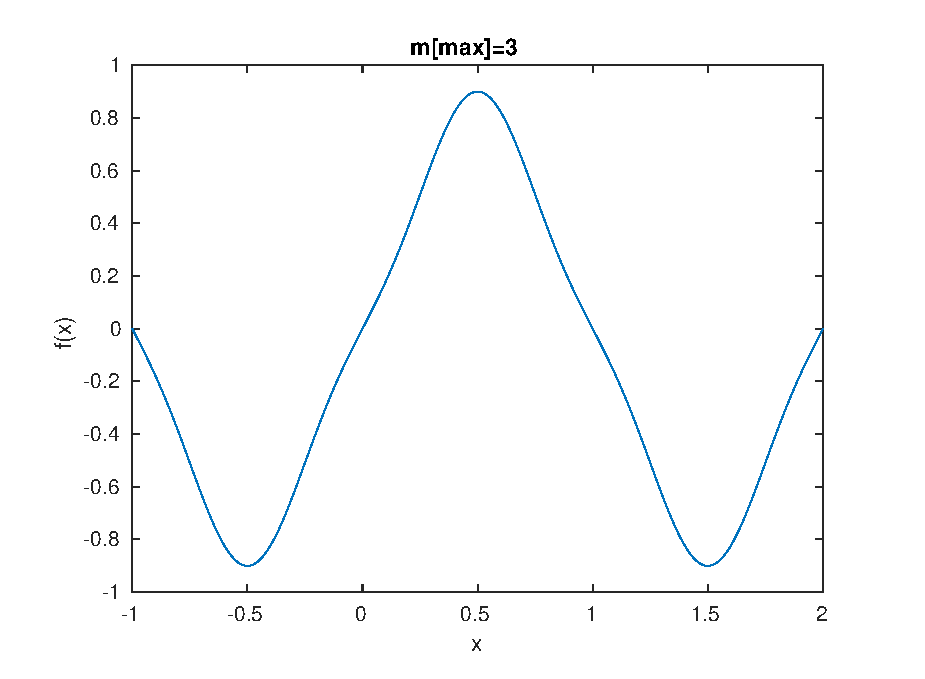
\includegraphics[width=8cm]{max3.eps}
        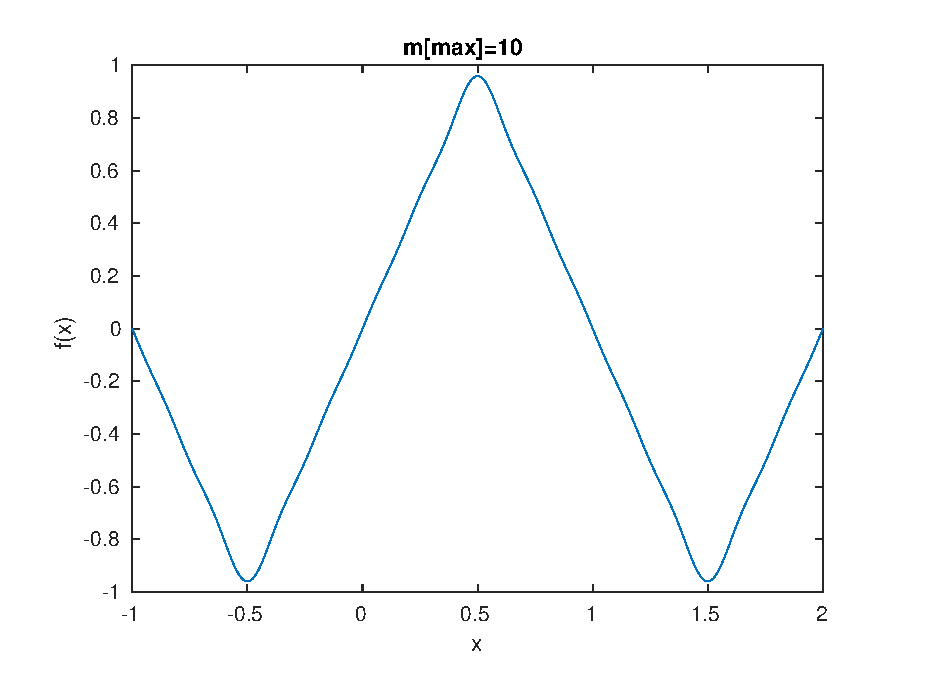
\includegraphics[width=8cm]{max10.eps}
        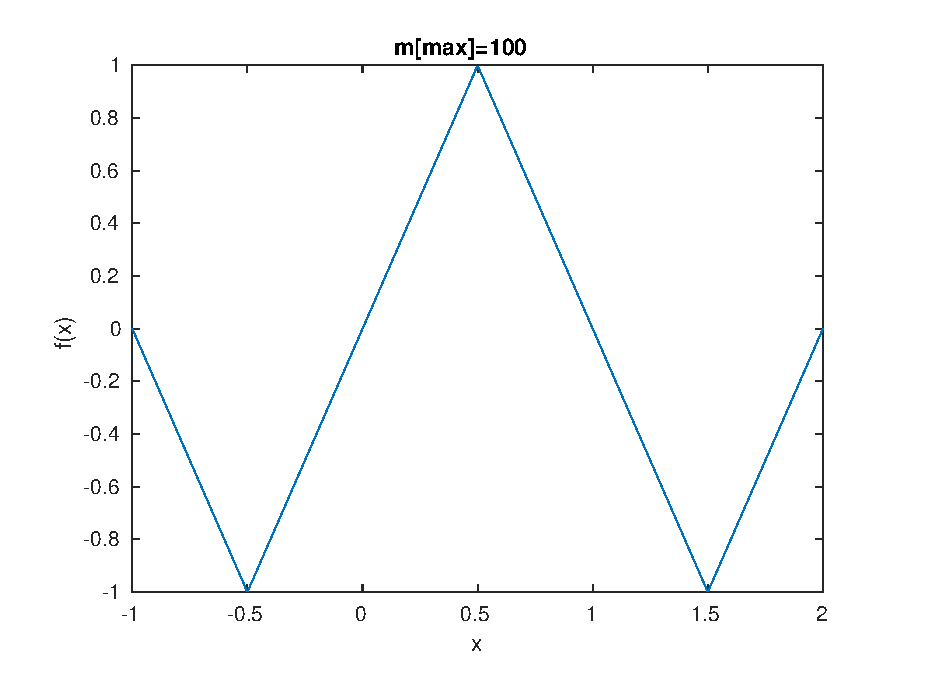
\includegraphics[width=8cm]{max100.eps}
\end{figure}



\end{document}


